%%%%%%%%%%%%%%%%%%%%%%%%%%%%%%%%%%%%%%%%%
% Beamer Presentation
% LaTeX Template
% Version 1.0 (10/11/12)
%
% This template has been downloaded from:
% http://www.LaTeXTemplates.com
%
% License:
% CC BY-NC-SA 3.0 (http://creativecommons.org/licenses/by-nc-sa/3.0/)
%
%%%%%%%%%%%%%%%%%%%%%%%%%%%%%%%%%%%%%%%%%

%----------------------------------------------------------------------------------------
%	PACKAGES AND THEMES
%----------------------------------------------------------------------------------------

%\documentclass[UTF8,aspectratio=169,14pt]{ctexbeamer}
\documentclass[UTF8,aspectratio=169]{ctexbeamer}
\usepackage{hyperref}
\hypersetup{
	colorlinks=true,
	linkcolor=red,
	anchorcolor=blue,
	citecolor=green
}

\mode<presentation> {
	
	% The Beamer class comes with a number of default slide themes
	% which change the colors and layouts of slides. Below this is a list
	% of all the themes, uncomment each in turn to see what they look like.
	
	%\usetheme{default}
	%\usetheme{AnnArbor}
	%\usetheme{Antibes}
	%\usetheme{Bergen}
	%\usetheme{Berkeley}
	%\usetheme{Berlin}
	%\usetheme{Boadilla}
	%\usetheme{CambridgeUS}
	%\usetheme{Copenhagen}
	%\usetheme{Darmstadt}
	%\usetheme{Dresden}
	%\usetheme{Frankfurt}
	%\usetheme{Goettingen}
	%\usetheme{Hannover}
	%\usetheme{Ilmenau}
	%\usetheme{JuanLesPins}
	%\usetheme{Luebeck}
	\usetheme{Madrid}
	%\usetheme{Malmoe}
	%\usetheme{Marburg}
	%\usetheme{Montpellier}
	%\usetheme{PaloAlto}
	%\usetheme{Pittsburgh}
	%\usetheme{Rochester}
	%\usetheme{Singapore}
	%\usetheme{Szeged}
	%\usetheme{Warsaw}
	
	% As well as themes, the Beamer class has a number of color themes
	% for any slide theme. Uncomment each of these in turn to see how it
	% changes the colors of your current slide theme.
	
	%\usecolortheme{albatross}
	%\usecolortheme{beaver}
	%\usecolortheme{beetle}
	%\usecolortheme{crane}
	%\usecolortheme{dolphin}
	%\usecolortheme{dove}
	%\usecolortheme{fly}
	%\usecolortheme{lily}
	%\usecolortheme{orchid}
	%\usecolortheme{rose}
	%\usecolortheme{seagull}
	%\usecolortheme{seahorse}
	%\usecolortheme{whale}
	%\usecolortheme{wolverine}
	
	%\setbeamertemplate{footline} % To remove the footer line in all slides uncomment this line
	%\setbeamertemplate{footline}[page number] % To replace the footer line in all slides with a simple slide count uncomment this line
	
	%\setbeamertemplate{navigation symbols}{} % To remove the navigation symbols from the bottom of all slides uncomment this line
}

\usepackage{graphicx} % Allows including images
\graphicspath{{./figs/}}
\usepackage{booktabs} % Allows the use of \toprule, \midrule and \bottomrule in tables
\usepackage{longtable}
\usepackage{listings}
\usepackage{xcolor}
\lstset{numbers=left, %设置行号位置
	numberstyle=\tiny, %设置行号大小
	keywordstyle=\color{blue}, %设置关键字颜色
	commentstyle=\color[cmyk]{1,0,1,0}, %设置注释颜色
	frame=single, %设置边框格式
	escapeinside=``, %逃逸字符(1左面的键),用于显示中文
	%breaklines, %自动折行
	extendedchars=false, %解决代码跨页时,章节标题,页眉等汉字不显示的问题
	xleftmargin=2em,xrightmargin=2em, aboveskip=1em, %设置边距
	tabsize=4, %设置tab空格数
	showspaces=false %不显示空格
}
% Fonts
% \usepackage{libertine}
% \setmonofont{Courier}
\setCJKsansfont[ItalicFont=Noto Serif CJK SC Black, BoldFont=Noto Sans CJK SC Black]{Noto Sans CJK SC}
\setmainfont[Ligatures={Common,TeX}]{Linux  Libertine O}
\setmonofont[SmallCapsFont={Latin Modern Mono Caps}]{Latin Modern Mono Light}
\setsansfont{Linux Biolinum O}

\logo{
\includegraphics[width=0.55cm,height=0.55cm]{../../thcs-logo.png}}

%----------------------------------------------------------------------------------------
%	TITLE PAGE
%----------------------------------------------------------------------------------------

\title[第5讲]{第5讲 :The Interface of OS} % The short title appears at the bottom of every slide, the full title is only on the title page
\subtitle{第二节:Overview of POSIX }
\author{陈渝} % Your name
\institute[清华大学] % Your institution as it will appear on the bottom of every slide, may be shorthand to save space
{
	清华大学计算机系 \\ % Your institution for the title page
	\medskip
	\textit{yuchen@tsinghua.edu.cn} % Your email address
}
\date{\today} % Date, can be changed to a custom date


\begin{document}

\begin{frame}
\titlepage % Print the title page as the first slide
\end{frame}

%\begin{frame}
%\frametitle{提纲} % Table of contents slide, comment this block out to remove it
%\tableofcontents % Throughout your presentation, if you choose to use \section{} and \subsection{} commands, these will automatically be printed on this slide as an overview of your presentation
%\end{frame}
%
%%----------------------------------------------------------------------------------------
%%	PRESENTATION SLIDES
%%----------------------------------------------------------------------------------------
%
%%------------------------------------------------
%\section{第一节:课程概述} % Sections can be created in order to organize your presentation into discrete blocks, all sections and subsections are automatically printed in the table of contents as an overview of the talk
%%------------------------------------------------
%-------------------------------------------------
\begin{frame}[plain]
	\frametitle{Introduction}
	
	
	
	\begin{columns}
		
		\begin{column}{.4\textwidth}
			
			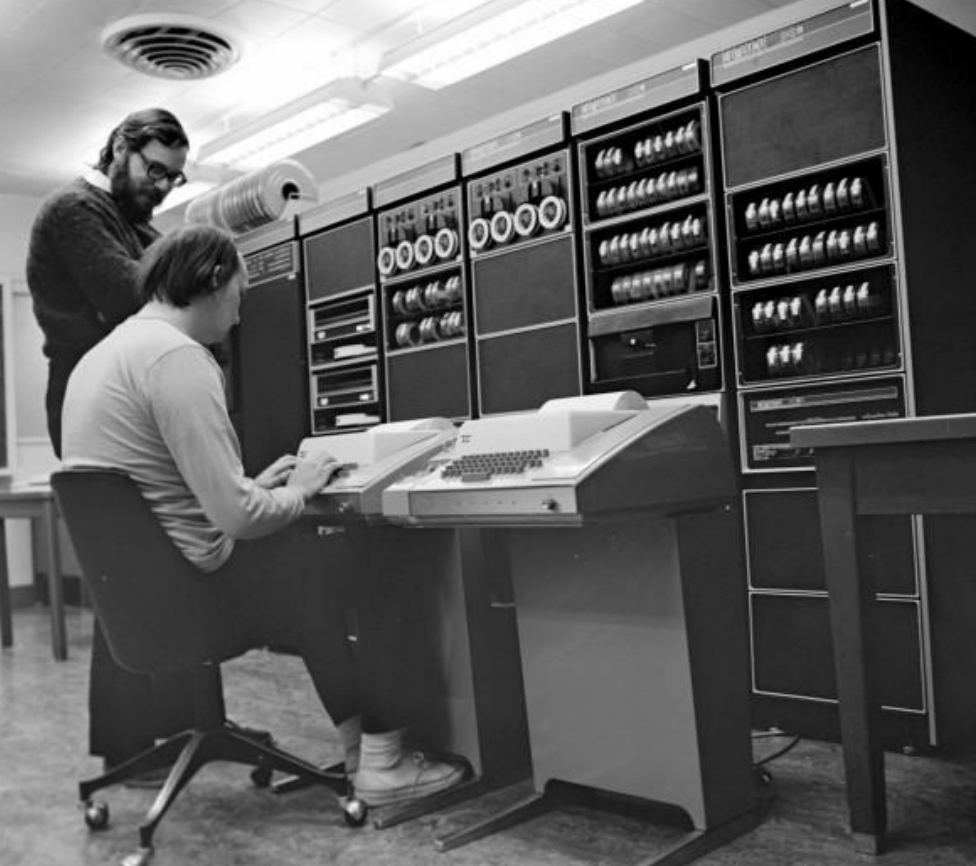
\includegraphics[width=1.\textwidth]{createunix}
			
		\end{column}
		
		\begin{column}{.6\textwidth}

		First Research Edition (1971)
		\begin{itemize}
			\item Complete rewrite (4213 lines kernel)
			\item Reference architecture
			
			\begin{itemize}
				\item 34 system calls
				\item 18 common with PDP-7 version
				\item 18 survive until today				
			\end{itemize}
			
			\item Binary code API
			\item Abstraction of standard I/O
			\item Devices as files
			
		\end{itemize}

	\begin{flushleft}
	\tiny Half Century of Unix:	History, Preservation, and	Lessons Learned, Diomidis Spinellis, 2017
	\\
	Analyzing a Decade of Linux System Calls, Mojtaba Bagherzadeh, etc. ICSE 2018
	
	
\end{flushleft}

		\end{column}
		
		
	\end{columns}
	

	
	
	
	
\end{frame}



%-------------------------------------------------
\begin{frame}[plain]
	\frametitle{Introduction}
	
	
	
	\begin{columns}
		
		\begin{column}{.2\textwidth}
			
			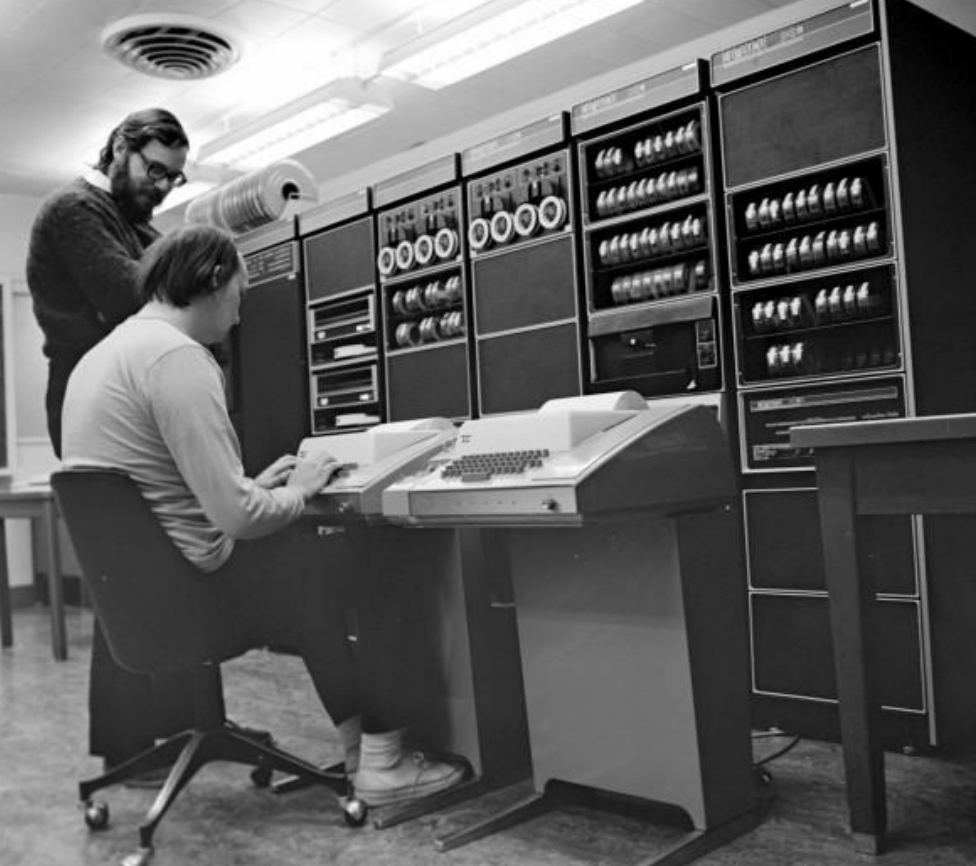
\includegraphics[width=1.\textwidth]{createunix}
			
		\end{column}
		
		\begin{column}{.8\textwidth}
			
			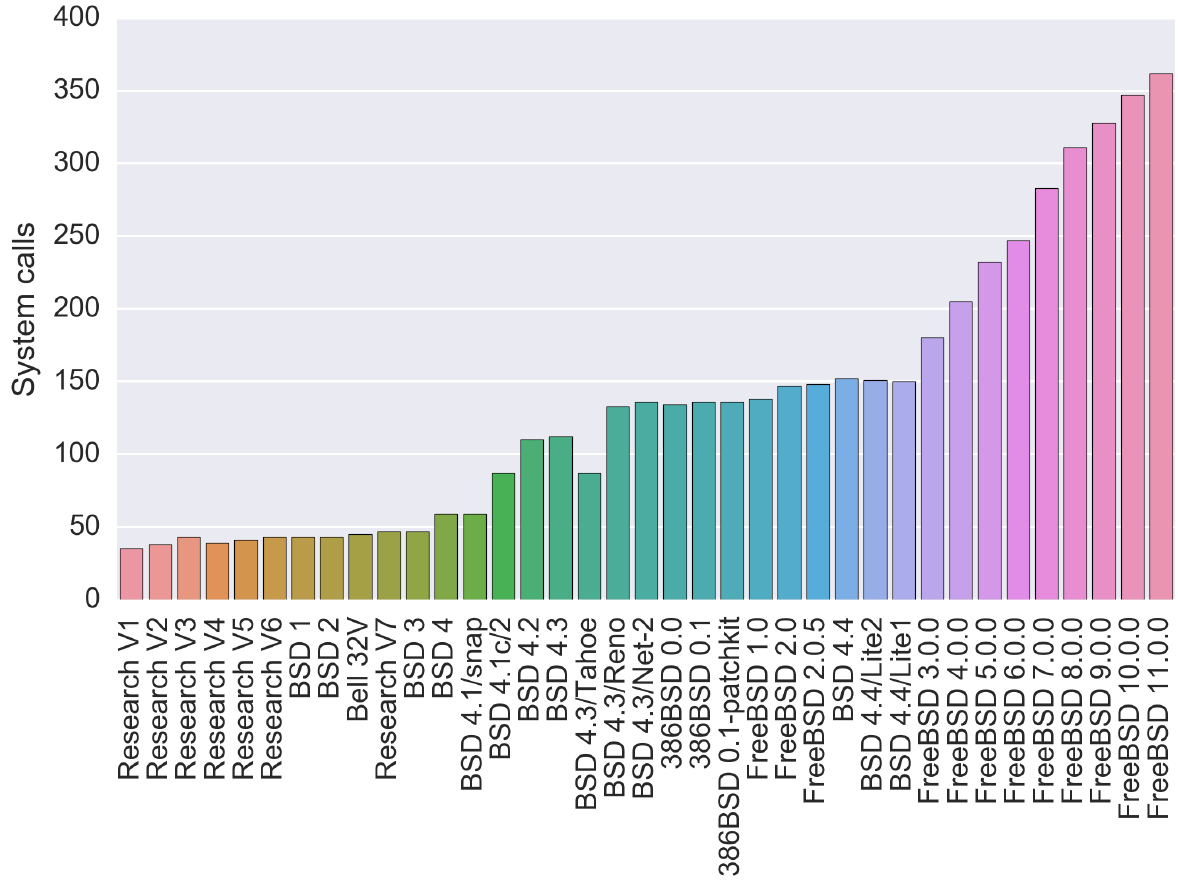
\includegraphics[width=.9\textwidth]{evolution-unix-syscall}

		\end{column}
		
		
	\end{columns}
	
	
\end{frame}

%-------------------------------------------------
\begin{frame}[plain]
	\frametitle{Introduction}
	
	
	
	\begin{columns}
		
		\begin{column}{.2\textwidth}
			
			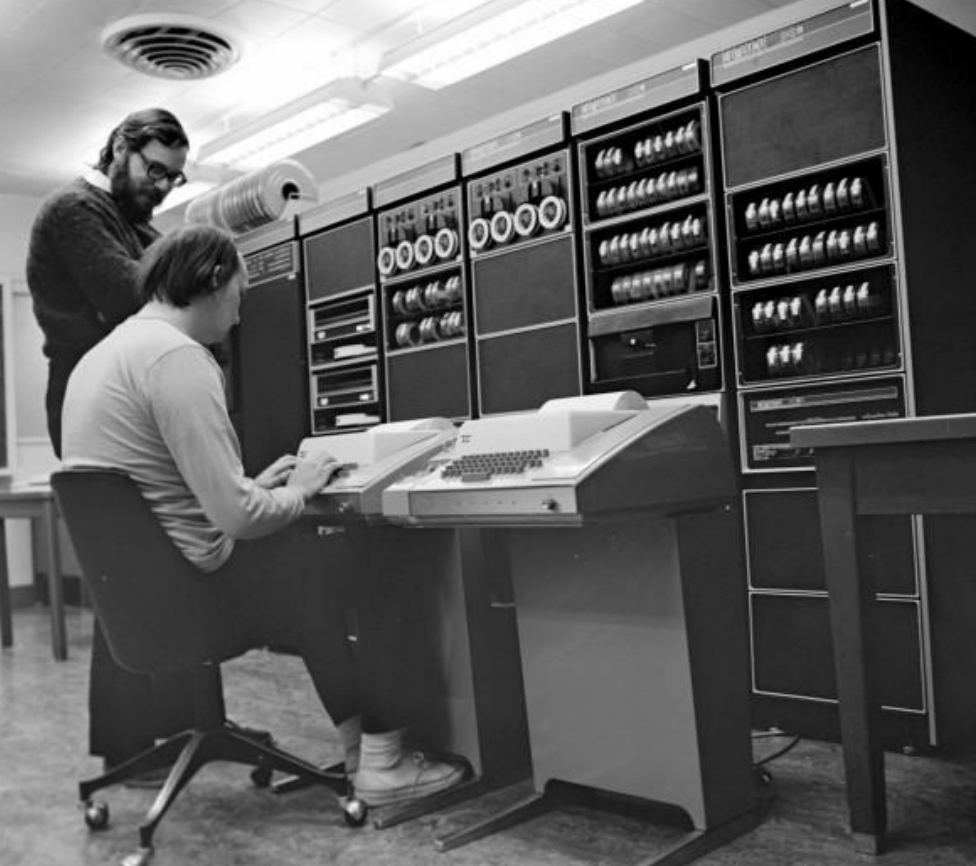
\includegraphics[width=1.\textwidth]{createunix}
			
		\end{column}
		
		\begin{column}{.8\textwidth}
			
			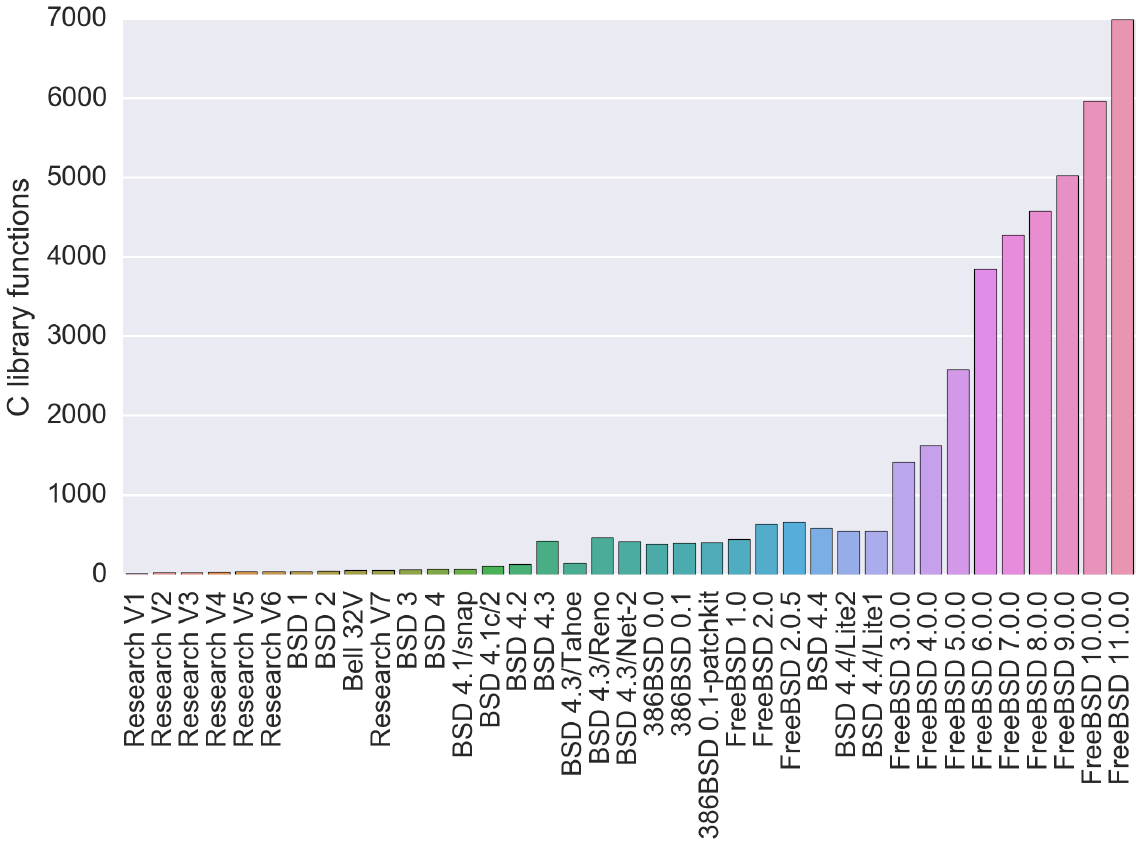
\includegraphics[width=.9\textwidth]{evolution-clib-funs}
			
		\end{column}
		
		
	\end{columns}
	
	
\end{frame}

%-------------------------------------------------
\begin{frame}[plain]
	\frametitle{Introduction -- The sequence of a system call}
	
	
	
			
			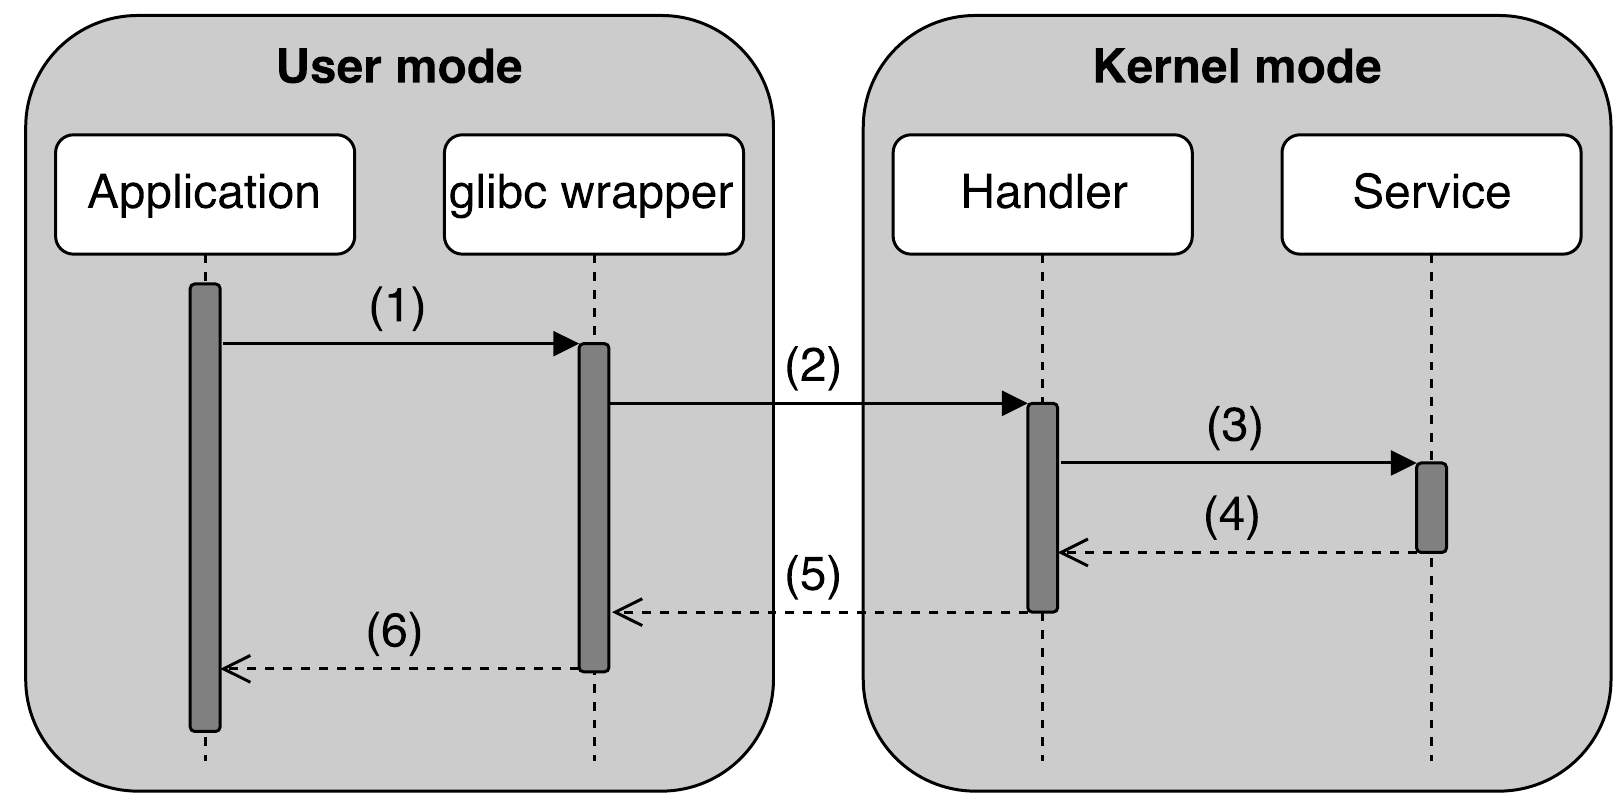
\includegraphics[width=1.\textwidth]{seq-syscall}
			

	
\end{frame}


%-------------------------------------------------
\begin{frame}[plain]
	\frametitle{Introduction -- An overview of syscall data collection}
	
	
	
	\centering
	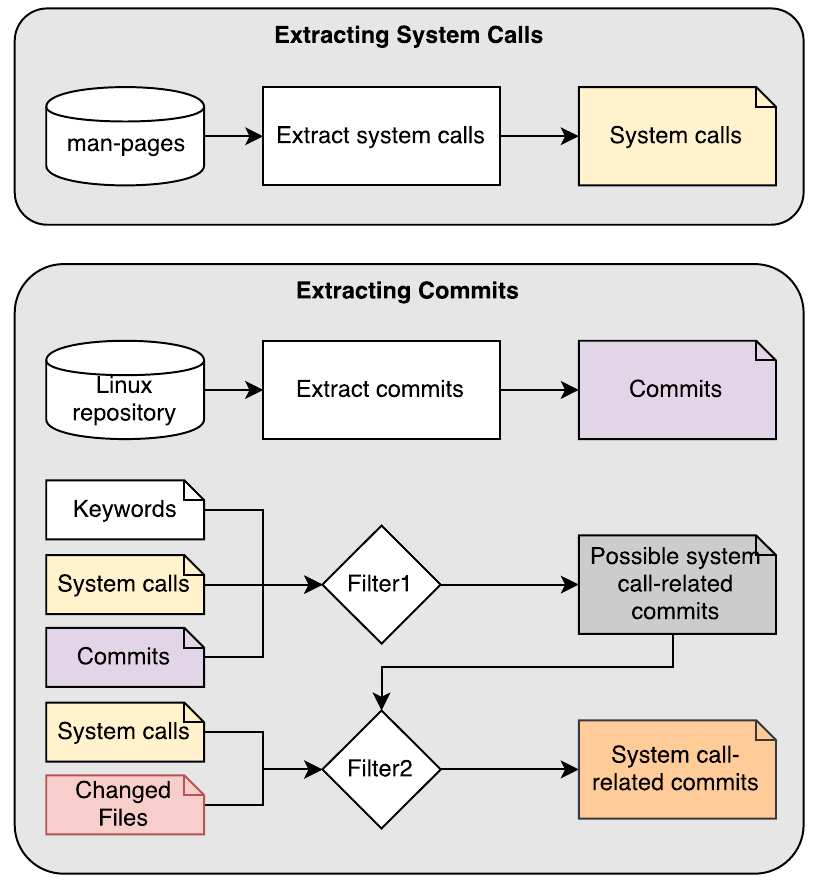
\includegraphics[width=.45\textwidth]{syscall-collect-data}
	
	
	
\end{frame}


%-------------------------------------------------
\begin{frame}[plain]
	\frametitle{Introduction -- An overview of syscall empirical study}
	
	
	
	\centering
	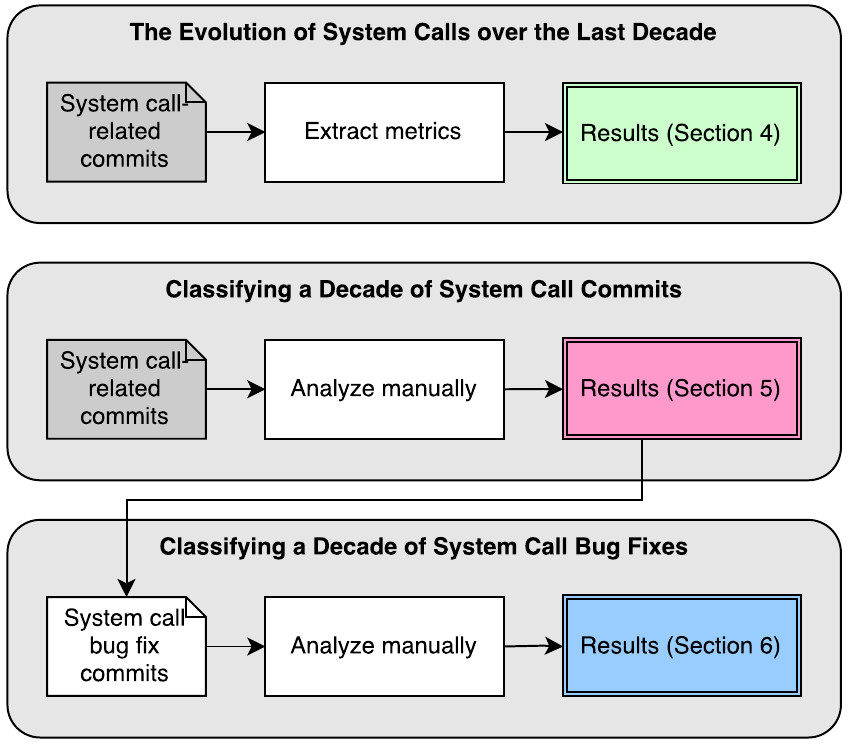
\includegraphics[width=.55\textwidth]{syscall-analyze-data}
	
	
	
\end{frame}



%-------------------------------------------------
\begin{frame}[plain]
	\frametitle{Introduction -- Syscall Categories}
	
	
	
	\centering
	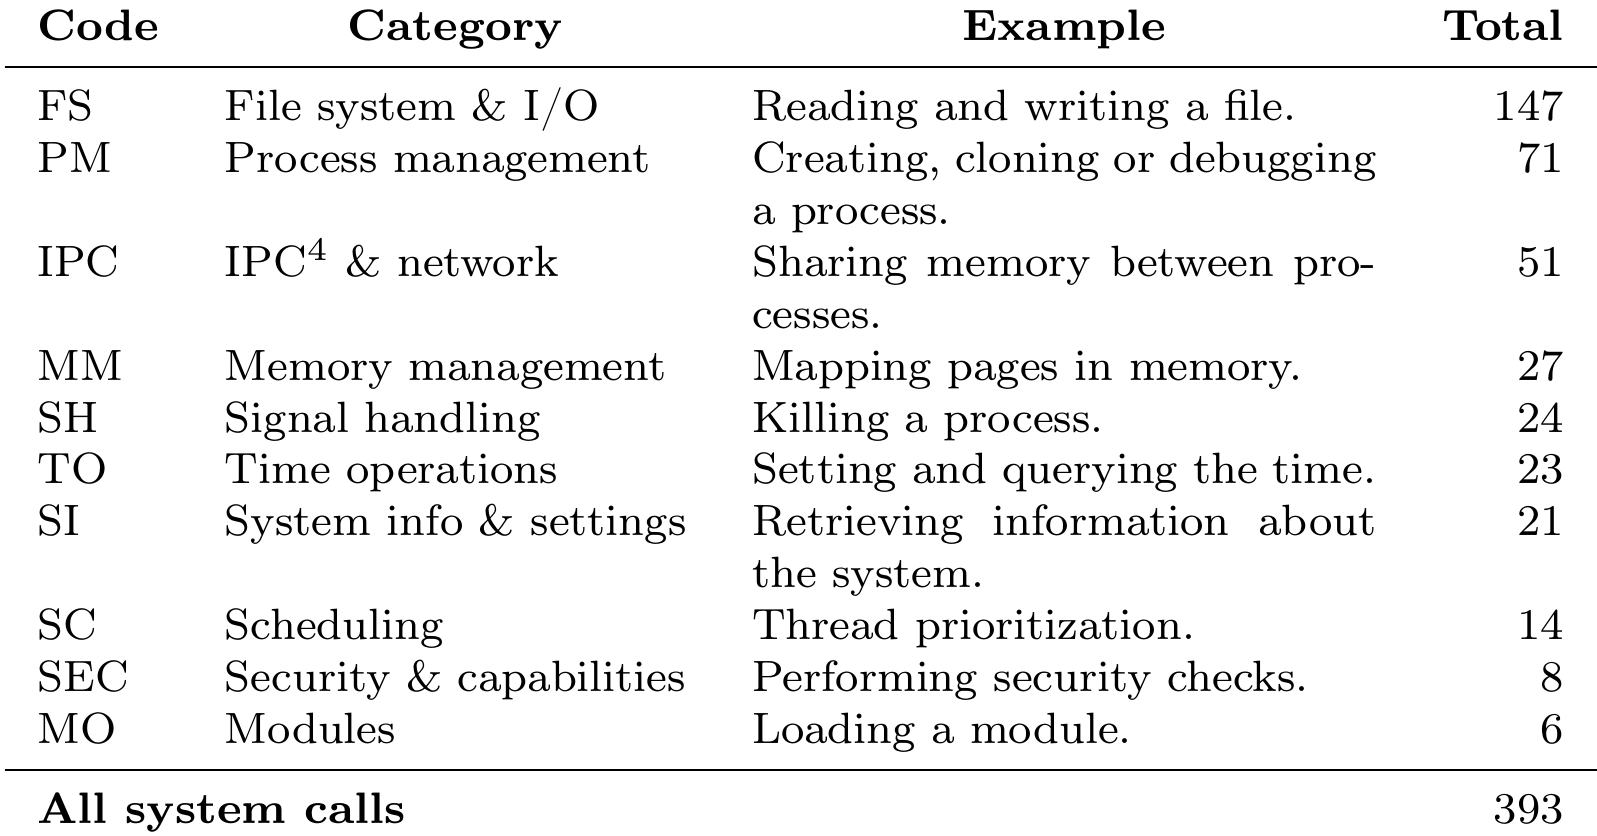
\includegraphics[width=.8\textwidth]{syscall-categories}
	
	
	
\end{frame}


%-------------------------------------------------
\begin{frame}[plain]
	\frametitle{Introduction -- sibling syscalls}
	
	
	
	\centering
	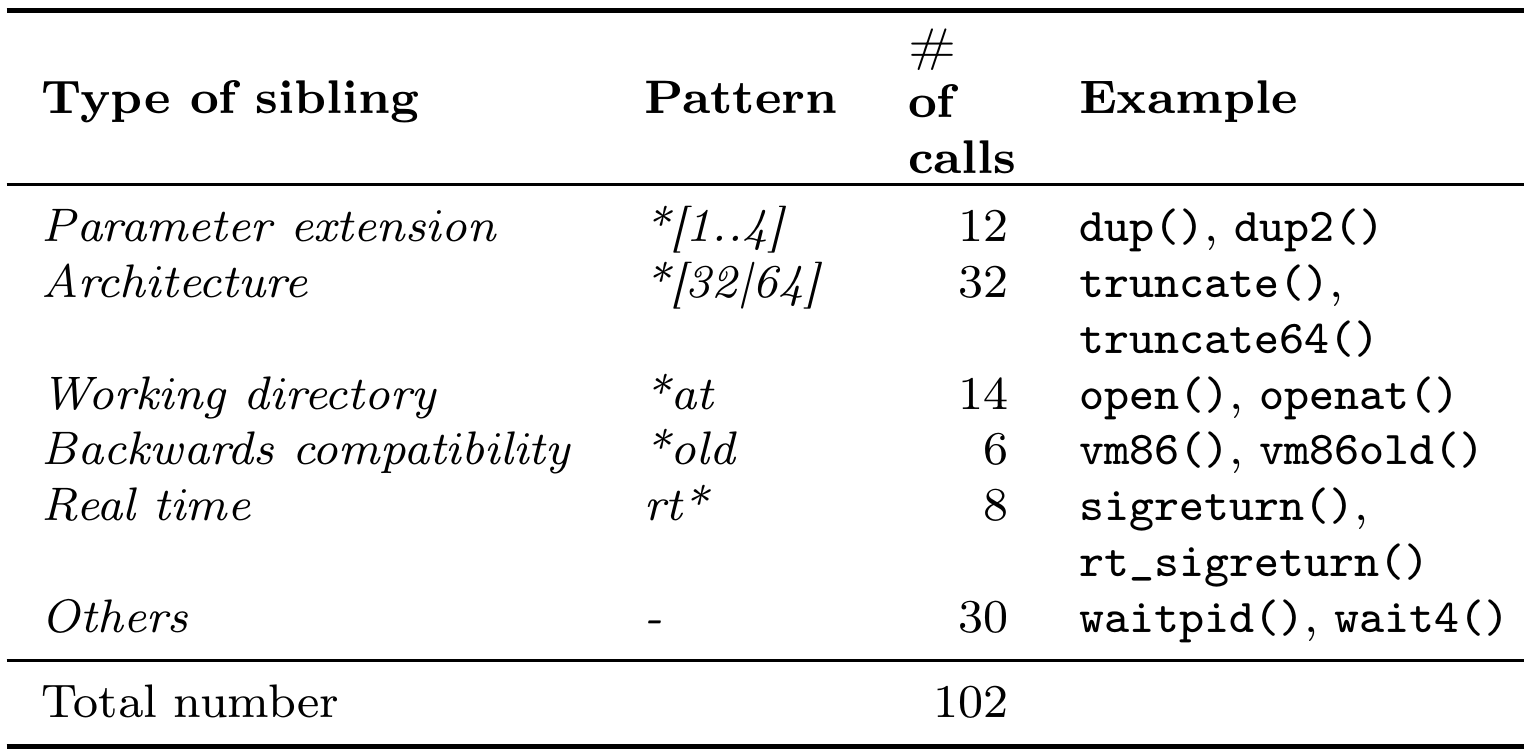
\includegraphics[width=.8\textwidth]{sibling-syscalls}
	
	
	
\end{frame}


%-------------------------------------------------
\begin{frame}[plain]
	\frametitle{Introduction -- new syscalls}
	
	
	
	\centering
	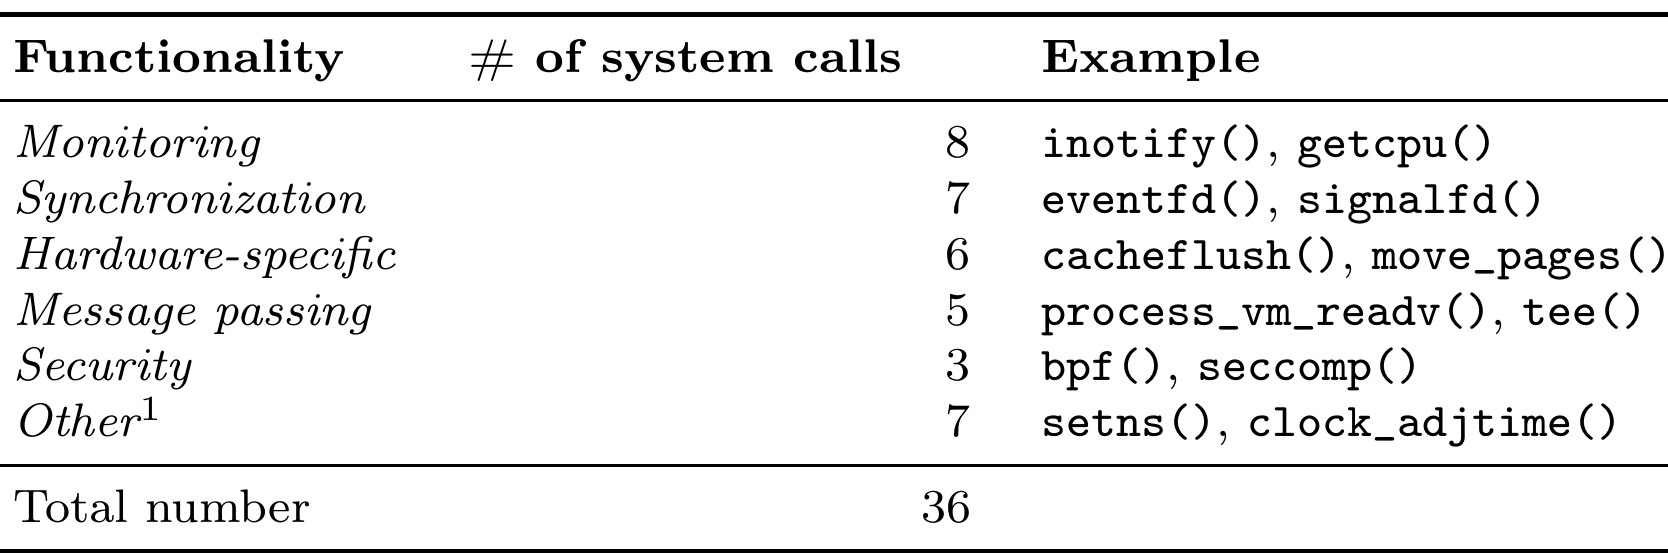
\includegraphics[width=.8\textwidth]{new-syscall}
	
	
	
\end{frame}


%-------------------------------------------------
\begin{frame}[plain]
	\frametitle{Introduction -- Classifying a Decade of System Call Commits}
	
	
	
	\centering
	\begin{itemize}\Large
		\item \textbf{Add/remove}: The commit was made to add or remove one or more system
		calls.
		
		\item \textbf{Bug fix}: The commit was made to fix a bug.
		\item \textbf{Improvement}: The commit was made to make an improvement.
		\item \textbf{Restructuring}: The commit was made to conduct code restructuring,
		such as cleaning up comments or refactoring.
		
	\end{itemize}
	
	
	
\end{frame}


%-------------------------------------------------
\begin{frame}[plain]
	\frametitle{Introduction -- The system calls with the most commits}
	
	
	
	\centering

	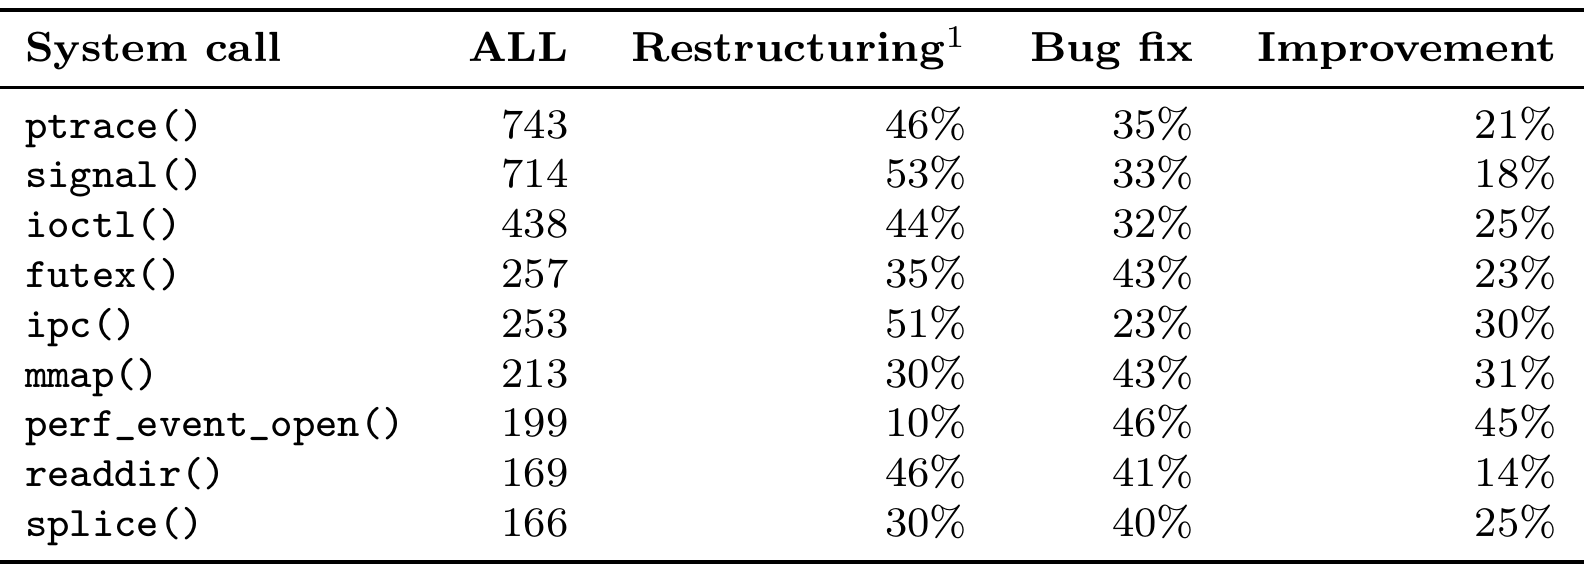
\includegraphics[width=1.\textwidth]{most-commits-syscall}

	
	
	
\end{frame}


%-------------------------------------------------
\begin{frame}[plain]
	\frametitle{Introduction -- Classifying  Bug Fixes for Sysalls}
	
	
	
%	\centering
	\begin{itemize}\large
		\item \textbf{Compatibility}: Compatibility-related bugs are caused by compatibility
		issues between architectures (e.g., 32-bit versus 64-bit).
		
		
		\item \textbf{Concurrency}: Concurrency-related bugs are caused by issues with atom-
		icity, execution order, synchronization or locking, and lead to problems
		such as deadlock or race conditions.
		\item \textbf{Error code}: Error code-related bugs are caused by returning the wrong
		error code or handling a returned error code incorrectly.
		\item \textbf{Memory}: Memory-related bugs are caused by incorrect usage of the mem-
		ory, thereby introducing an issue such as a memory leak.
		\item \textbf{Semantic} : Semantic bugs are bugs in the implementation of the system
		call-specific behaviour, such as the logic of the service provided by the
		system call.
		
		
	\end{itemize}
	
	Signal handling system calls have the highest number of semantic
	(9.33) and compatibility-related (1.70) bug fixes per system call.
	
\end{frame}


%-------------------------------------------------
\begin{frame}[plain]
	\frametitle{Introduction -- Classifying  Bug Fixes for Sysalls}
	
	
	
		\centering
	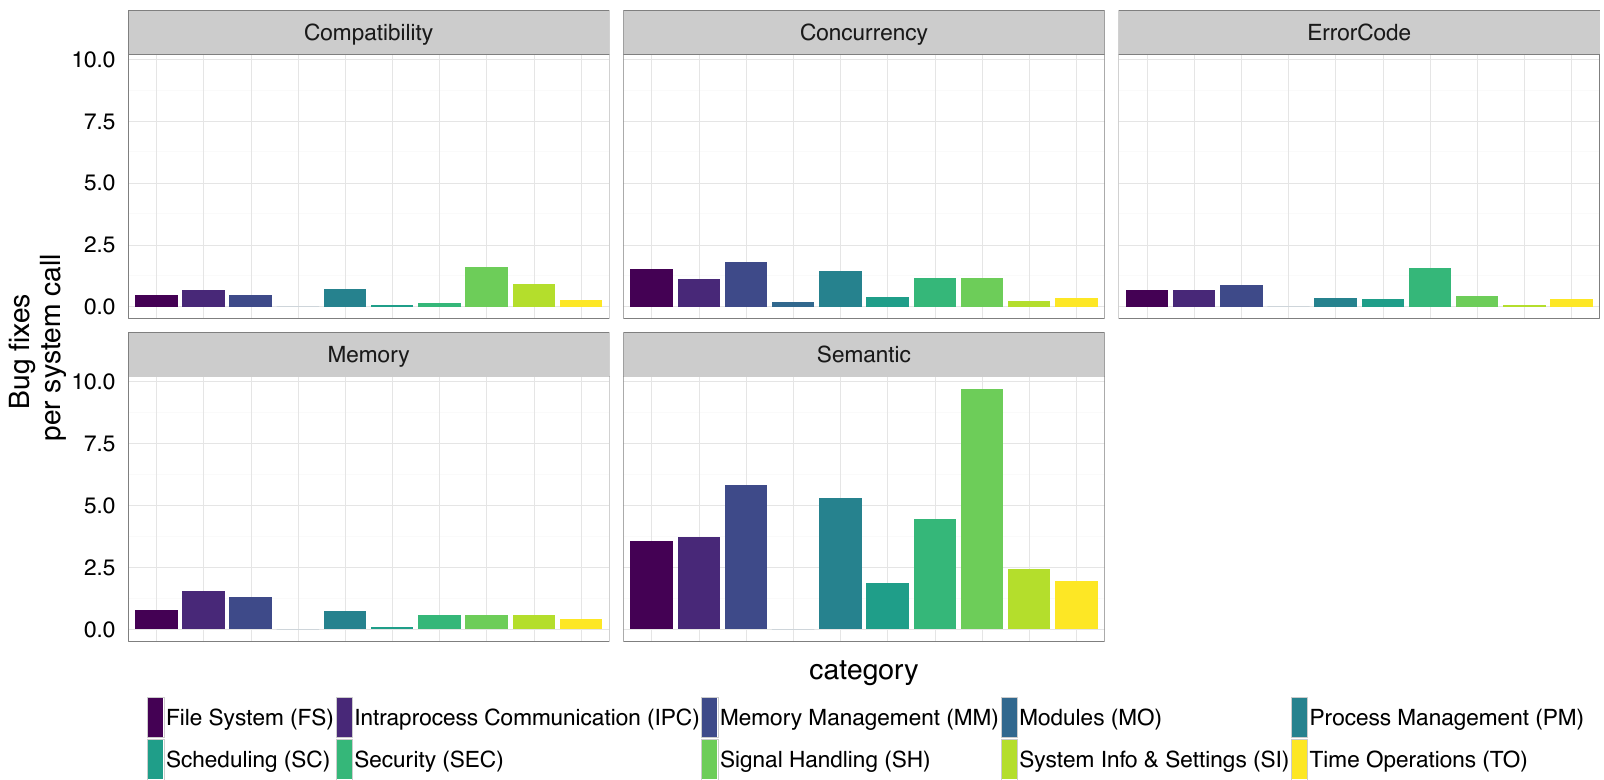
\includegraphics[width=.9\textwidth]{syscall-bugs}
	
	Signal handling system calls have the highest number of semantic
	(9.33) and compatibility-related (1.70) bug fixes per system call.
	
\end{frame}
%-----------
%-------------------------------------------------


%-------------------------------------------------

%-------------------------------------------------
\end{document}